\chapter{Aligning the interferometer}

\section{Introduction}
The Angular Sensing and Control (ASC) subsystem uses a set of quadrant
photodiodes, RF electronics, digital filters, and coil actuators to
both sense and correct for the angular motion of the interferometer
mirrors. Requirements for performance are stringent as too little
control increases the susceptibility to lock losses and too much
control decreases the interferometer's strain sensitivity. This
chapter will lay out the foundations for understanding angular sensing
and control in the context of Enhanced LIGO and Chapter 5 will present
the results of a set of measuremets characterizing the Enhanced LIGO ASC
performance. 



\subsection{Layout}
There are four main subsets of sensor systems for the ASC:
\begin{itemize}
\item wavefront sensors (WFS1, WFS2, WFS3, WFS4) \vspace{-10pt}
\item quadrant photodiodes (QPDX, QPDY) \vspace{-10pt}
\item optical levers (MMT3, RM, BS, ITMX, ITMY, ETMX, ETMY) \vspace{-10pt}
\item camera image (BS)
\end{itemize}
All but the wavefront sensors provide quite straightforward measures
of angular motion. The optical levers are local to each
large optic, for instance, and provide a record at all times of pitch and yaw
pointing of each mirror with respect to the ground. The video camera
monitors the location of the spot on the beam splitter,
thus serving as a sensor of the directionality of the input beam. The
two QPDs look at the light transmitted through each arm cavity,
indicating the modal axis of each cavity.

Finally, the wavefront sensors provide the most sophisticated 


The most primitive sensor is that of the physical video camera. The
image of the speckle of light reflected off of the beam splitter (see
Fig. \ref{fig:BCS}) is fed into a labview program which integrates the
intensity of the image to identify the coordinates of the center of
the beam spot. This is compared with a hardcoded desired center
location and a mirror upstream (MMT1) is moved to redirect the input
beam, minimizing the difference between the desired and actual beam
spot location on the BS.

\begin{figure}
\begin{centering}
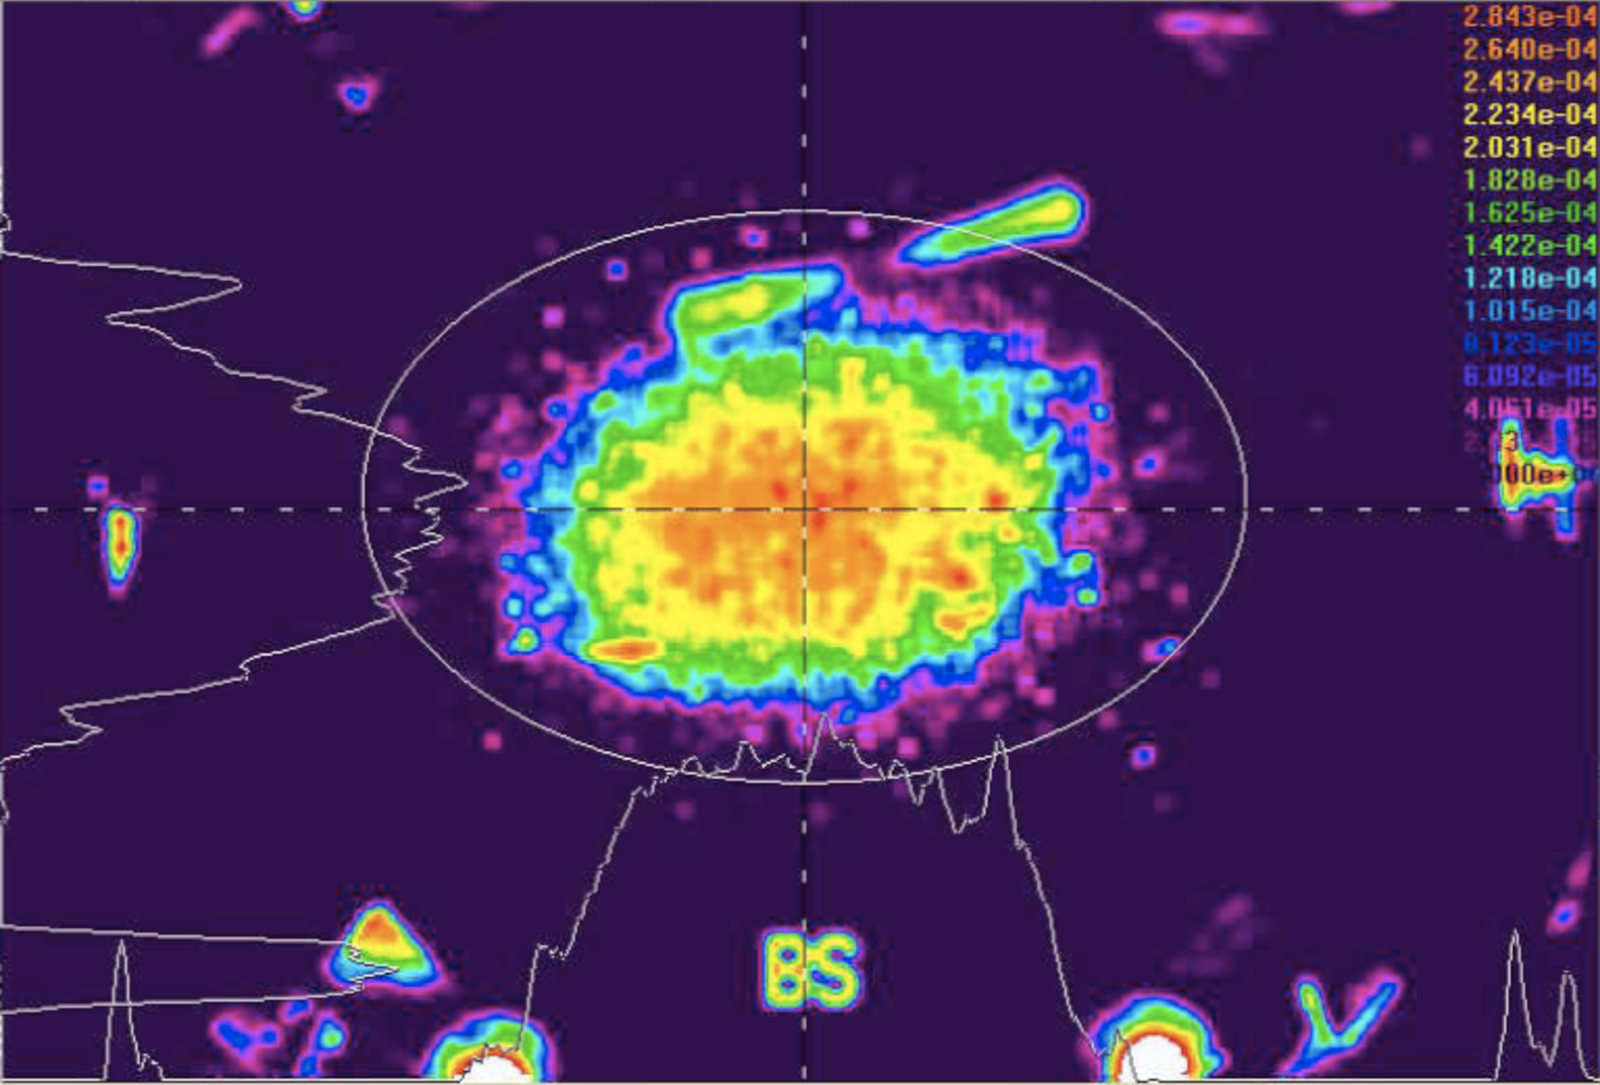
\includegraphics[width=0.8\textwidth]{figures/BCSspiricon.pdf}
\caption{Image of beam on beam splitter as used for the beam centering servo.}
\label{fig:BCS}
\end{centering}
\end{figure}

\subsection{Optical levers}
The optical lever is a HeNe laser beam that reflects off of the mirror
and onto a QPD. Both the laser and QPD are mounted on heavy piers to
reduce the seismic noise contribution to the QPD signal. The purpose
of the optical lever is to sense the mirror's motion relative to the
ground and to provide a feedback signal to the mirror's coils to reduce
the sensed motion. Each large optic has its own independent optical
lever loop which is almost always on, even when the interferometer is
out of lock. The optical lever loops provide the second level of
controlled stabilization of the mirrors, after only the local
damping. 


\begin{itemize}
\item layout
\item loopology
\item role of optical levers
\end{itemize}

\section{Wave-front Sensors}
\begin{itemize}
\item hardware
\item theory
\end{itemize}

\section{Cavities with radiation pressure}
\begin{itemize}
\item cavity eigenfunctions
\item mirror torque
\item cavity misalignment
\item opto-mechanical transfer functions
\item hard and soft modes
\item Eiichi's work
\end{itemize}

\section{Enhanced LIGO ASC design}
\begin{itemize}
\item change of basis (Lisa's work)
\item filters
\end{itemize}

